\documentclass{article}
\usepackage{listings}
\usepackage{mathrsfs}
\usepackage[utf8]{inputenc}
\usepackage{amssymb}
\usepackage{lipsum}
\usepackage{amsmath}
\usepackage{fancyhdr}
\usepackage{geometry}
\usepackage{scrextend}
\usepackage[english,german]{babel}
\usepackage{titling}
\setlength{\droptitle}{-3cm}
\usepackage{tikz}
\usepackage{algorithm,algpseudocode}
\usepackage[doublespacing]{setspace}
\usetikzlibrary{datavisualization}
\usetikzlibrary{datavisualization.formats.functions}
\usepackage{polynom}
\usepackage{amsmath}
\usepackage{gauss}
\usepackage{tkz-euclide}
\usepackage{minted}
\usetikzlibrary{datavisualization}
\usetikzlibrary{datavisualization.formats.functions}
\author{
Alexander Mattick Kennung: qi69dube\\
Kapitel 1
}
\usepackage{import}
\date{\today}
\geometry{a4paper, margin=2cm}
\usepackage{stackengine}
\parskip 1em
\newcommand\stackequal[2]{%
  \mathrel{\stackunder[2pt]{\stackon[4pt]{=}{$\scriptscriptstyle#1$}}{%
  $\scriptscriptstyle#2$}}
 }
\makeatletter
\renewcommand*\env@matrix[1][*\c@MaxMatrixCols c]{%
  \hskip -\arraycolsep
  \let\@ifnextchar\new@ifnextchar
  \array{#1}}
\makeatother
\lstset{
  language=haskell,
}
\lstnewenvironment{code}{\lstset{language=Haskell,basicstyle=\small}}{}
\usepackage{enumitem}
\setlist{nosep}
\usepackage{titlesec}
\usepackage{ stmaryrd }
\usepackage{verbatim}
\usepackage{tikz-qtree}
\usepackage{bussproofs}

\titlespacing*{\subsection}{0pt}{2pt}{3pt}
\titlespacing*{\section}{0pt}{0pt}{5pt}
\titlespacing*{\subsubsection}{0pt}{1pt}{2pt}
\title{Übung 7}


\begin{document}
	\maketitle
	ZV X und Y sind unabhängige, gleichverteilte ZV aus $\mathcal{U}(a,b)$\\
	also ist
	\[f^Y(y)=\frac{1}{b-a}1_{(a,b)}\]
	\[f^X(x)=\frac{1}{b-a}1_{(a,b)}\]
	Dazu die Faltung $Z=X+Y$ wobei $z=x+y\in (a,2b)$:
	\[f^{(X+Y)}(z)=\int^\infty_{-\infty}f^Y(y)f^X(z-y)dy\]
	\[f^{(X+Y)}(z)=\int^\infty_{-\infty}\frac{1}{b-a}1_{(a,b)}(y)\frac{1}{b-a}1_{(a,b)}(z-y)dy\]
	\[f^{(X+Y)}(z)=\frac{1}{(b-a)^2}\int^\infty_{-\infty}1_{(a,b)}(y)1_{(a,b)}(z-y)dy\]
	Die letzte Indikatorfunktion liefert $1_{(a,b)}(z-y)\iff z-y\in(a,b) \iff y\in (z-b,z-a)\iff 1_{(z-b,z-a)}(y)$ (weil $z-y=x\in(a,b)\iff y = z-x$, grenzen drehen sich um, weil ich das element der Menge minus nehme).\\
	\[\frac{1}{(b-a)^2}\int^\infty_{-\infty}1_{(a,b)}(y)1_{(z-b,z-a)}(y)dy\iff \frac{1}{(b-a)^2}\int^\infty_{-\infty}1_{(a,b)\cap (z-b,z-a)}(y)dy\]
	bzw $a<y<b \land z-b < y <z-a$\\
	daraus folgt, dass y mindestens $max(a,z-b)$ groß sein muss und höchstens $min(b,z-a)$.\\
	Der erste Randfall liefert $a<z-b\implies a+b<z$ für das untere Intervall, $z-a<b\implies z<a+b $
	für das obere.\\
	Explizit muss noch der fall von $a+b=z $ betrachtet werden.\\
	Da sowohl $f^X$ als auch $f^Y$ stetig in (a+b) sind, muss auch deren Produkt stetig sein.\\
	Somit können wir $a+b$ zu einem der Fälle hinzunehmen. (hier dem ersten)\\
	Es gilt $y\in (a,z-a)$ weil y mindestens a sein muss:\\
	daraus folgt $z\leq a+b \land y<z-a\implies z\leq a+b \land a<z-a\implies  z\in (2a,a+b]$\\
	Dieser Teilintegral:\\
	\[\int_a^{z-a}\frac{1}{(b-a)^2}dy = \frac{z-a}{(b-a)^2}-\frac{a}{(b-a)^2}=\frac{z-2a}{(b-a)^2}\]
	Wenn $z\in (a+b,2b)$ dann $ y\in (z-b,b)$ da y höchstens b werden kann.\\
	(herleitung analog)
	\[\int^b_{z-b}\frac{1}{(b-a)^2}dy = \frac{b}{(b-a)^2}-\frac{z-b}{(b-a)^2}\]

	somit erhalten wir insgesamt:
	\begin{equation*}
	f_Z(z) = \begin{cases}
	\frac{z-2a}{(b-a)^2}&z\in (2a,a+b]\\
	\frac{2b-z}{(b-a)^2}&z\in (a+b,2b)\\
	0 &sonst
	\end{cases}
	\end{equation*}
	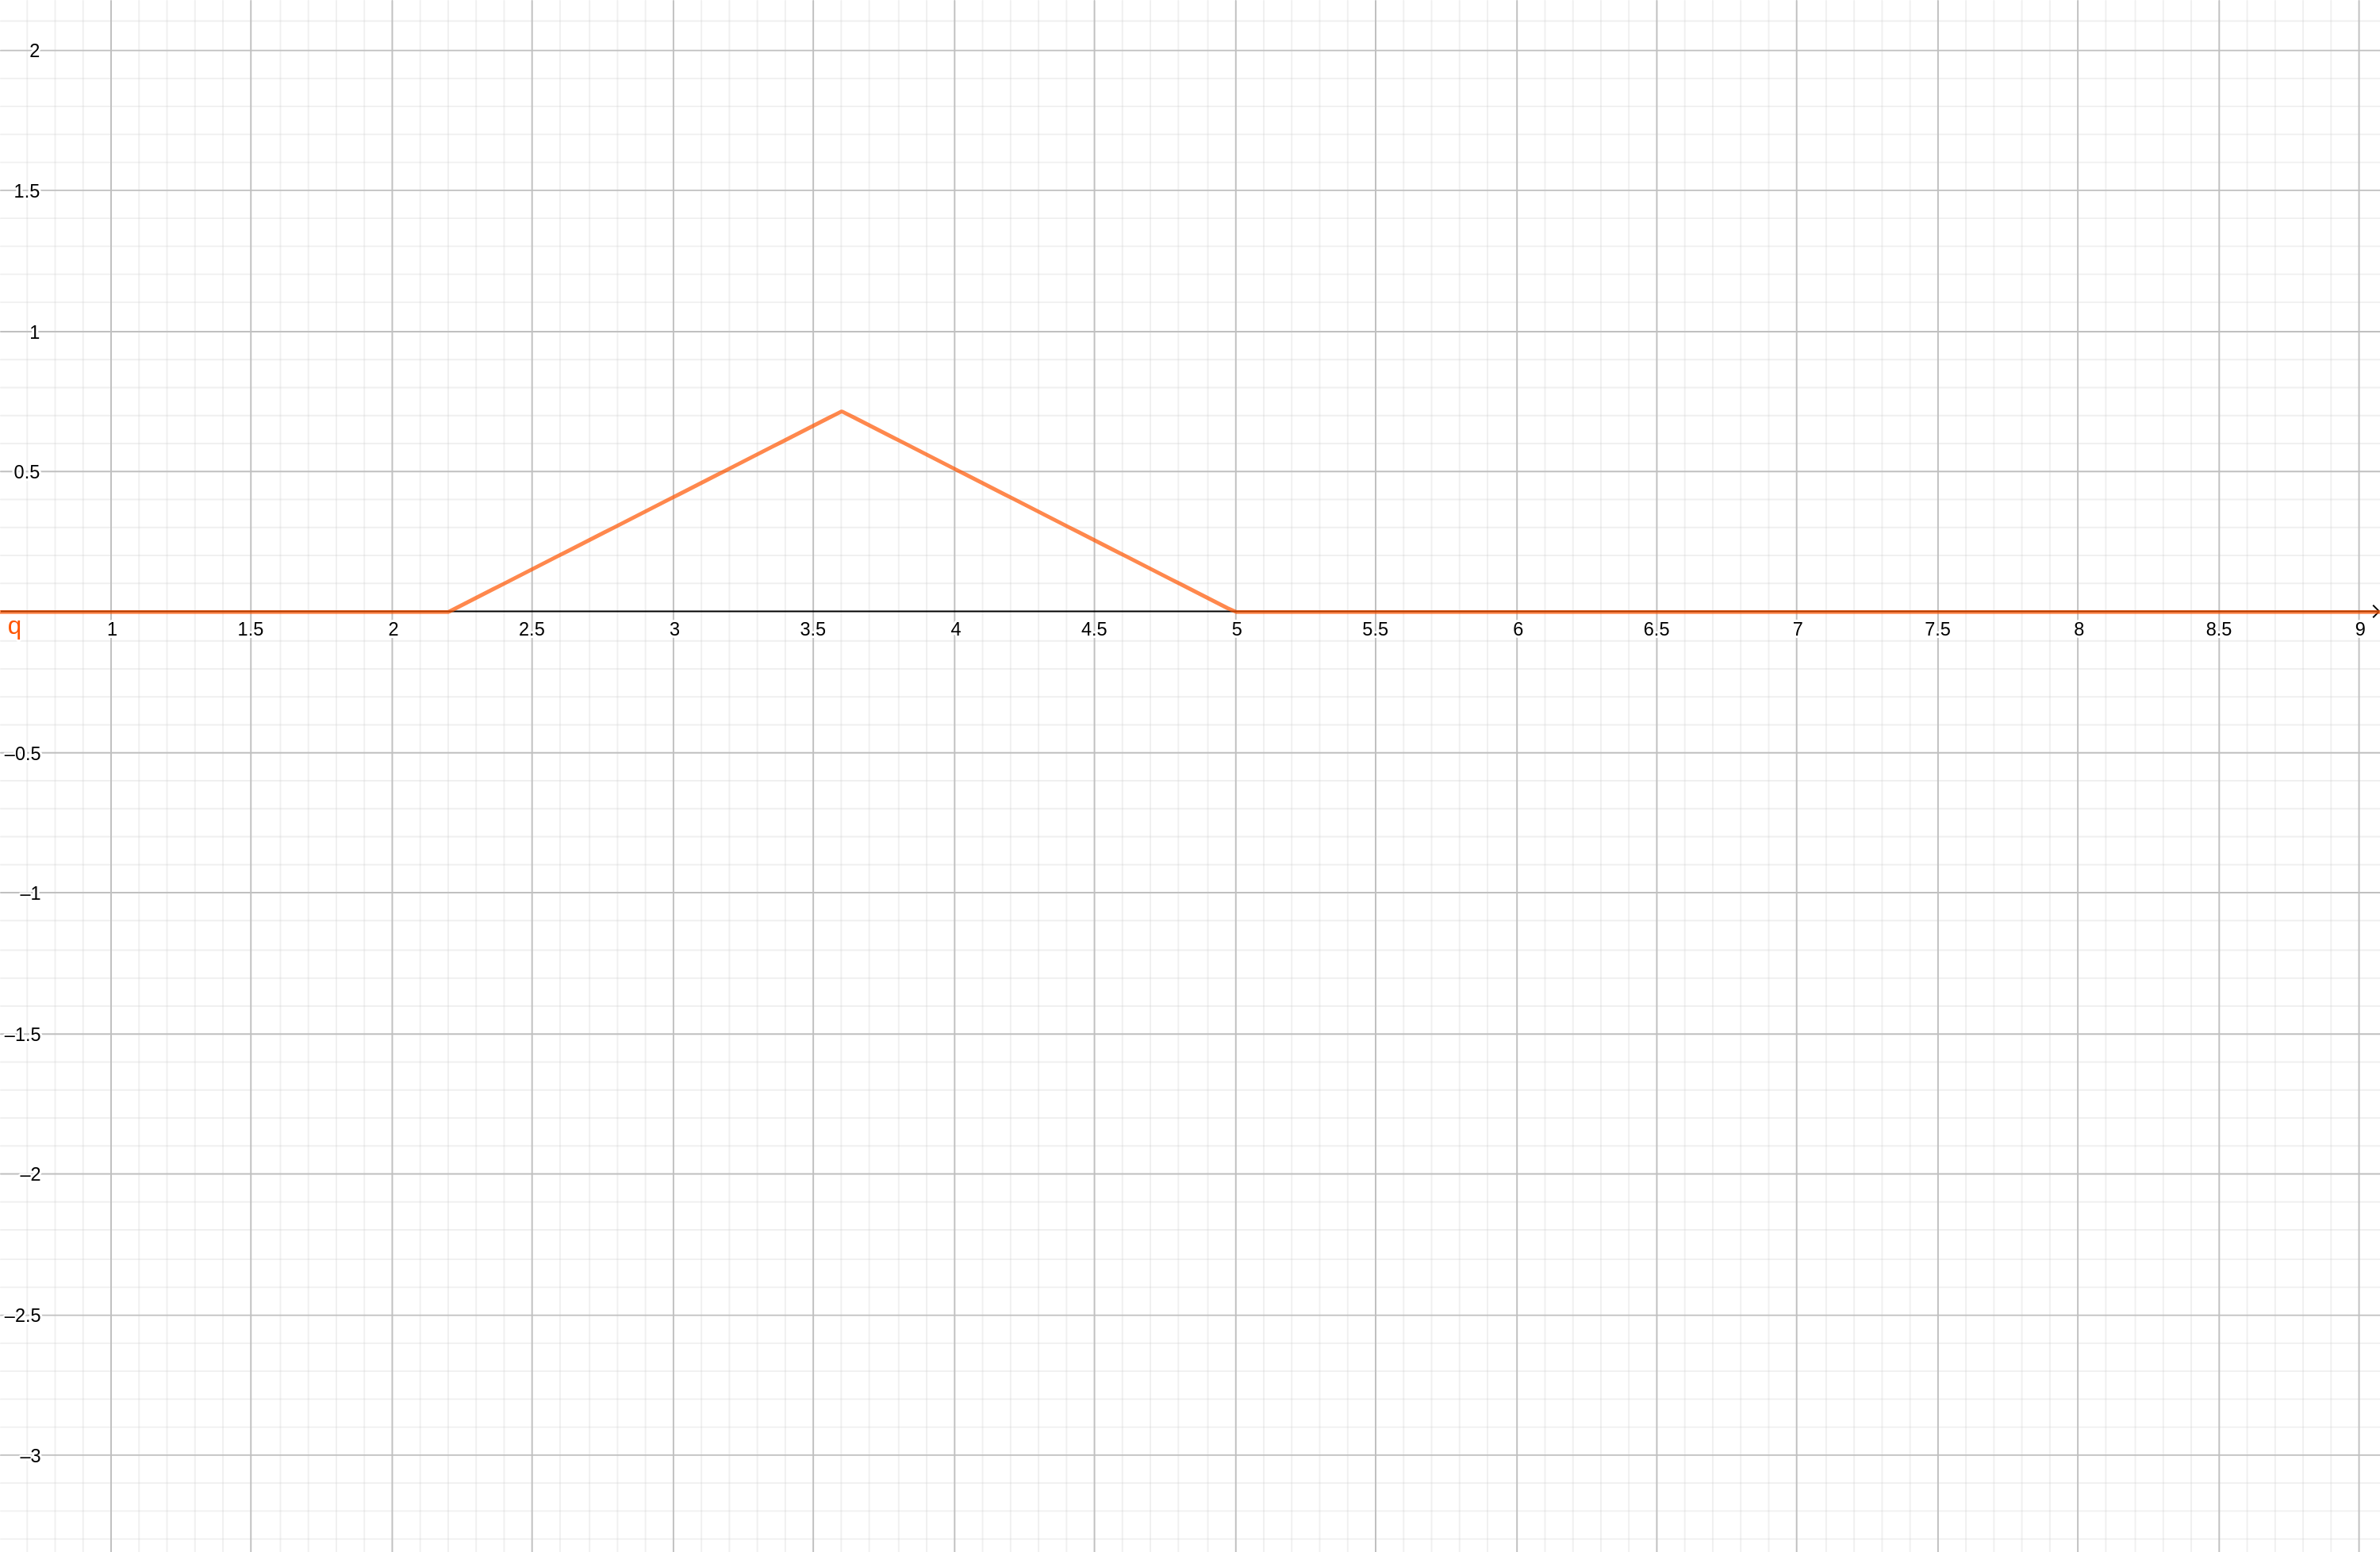
\includegraphics[width=256px]{skizzeHauptaufgabe.png}
	\section{}
	Der Träger ist $t_1^2+t_2^2\leq 1$ dies ist ein Kreis, somit kann die Verteilungsfunktion nicht stochastisch unabhängig sein.\\
	Umformung nach $t_1^2$ liefert $t_1^2\leq 1-t_2^2$, da $t_1\in\mathbb{R}$
	\[f^{X}(t_2)=\int_{-\sqrt{1-t_2^2}}^{\sqrt{1-t_2^2}} f(t_1,t_2)dt_1 \]
	\[f^{X}(t_2)=\int_{-\sqrt{1-t_2^2}}^{\sqrt{1-t_2^2}} \frac{1}{\pi}dt_1 \]
	\[f^{X}(t_2)= [\frac{1}{\pi}t_1]_{-\sqrt{1-t_2^2}}^{\sqrt{1-t_2^2}} \]
	\[f^{X}(t_2)= \frac{1}{\pi}(\sqrt{1-t_2^2}) - (-\frac{1}{\pi}(\sqrt{1-t_2^2})) \]
	\[f^{X}(t_2)= \frac{2}{\pi}(\sqrt{1-t_2^2}) \]
	analog für y\\
	\[f^{Y}(t_1)=\int_{-\sqrt{1-t_1^2}}^{\sqrt{1-t_1^2}} f(t_1,t_2)dt_2 \]
	\[f^{Y}(t_1)=\int_{-\sqrt{1-t_1^2}}^{\sqrt{1-t_1^2}} \frac{1}{\pi}dt_2 \]
	\[f^{Y}(t_1)=\frac{1}{\pi}(\sqrt{1-t_1^2})- (-\frac{1}{\pi}(\sqrt{1-t_1^2}))\]
	\[f^{Y}(t_1)=\frac{2}{\pi}(\sqrt{1-t_1^2})\]
	bei beiden gilt $t_{1/2}\in [0,1]$\\
	Das produkt von $f^{X}(0)f^{Y}(0) =\frac{4}{\pi^2}\neq f^{(X,Y)}(0,0) =\frac{1}{\pi}$\\
	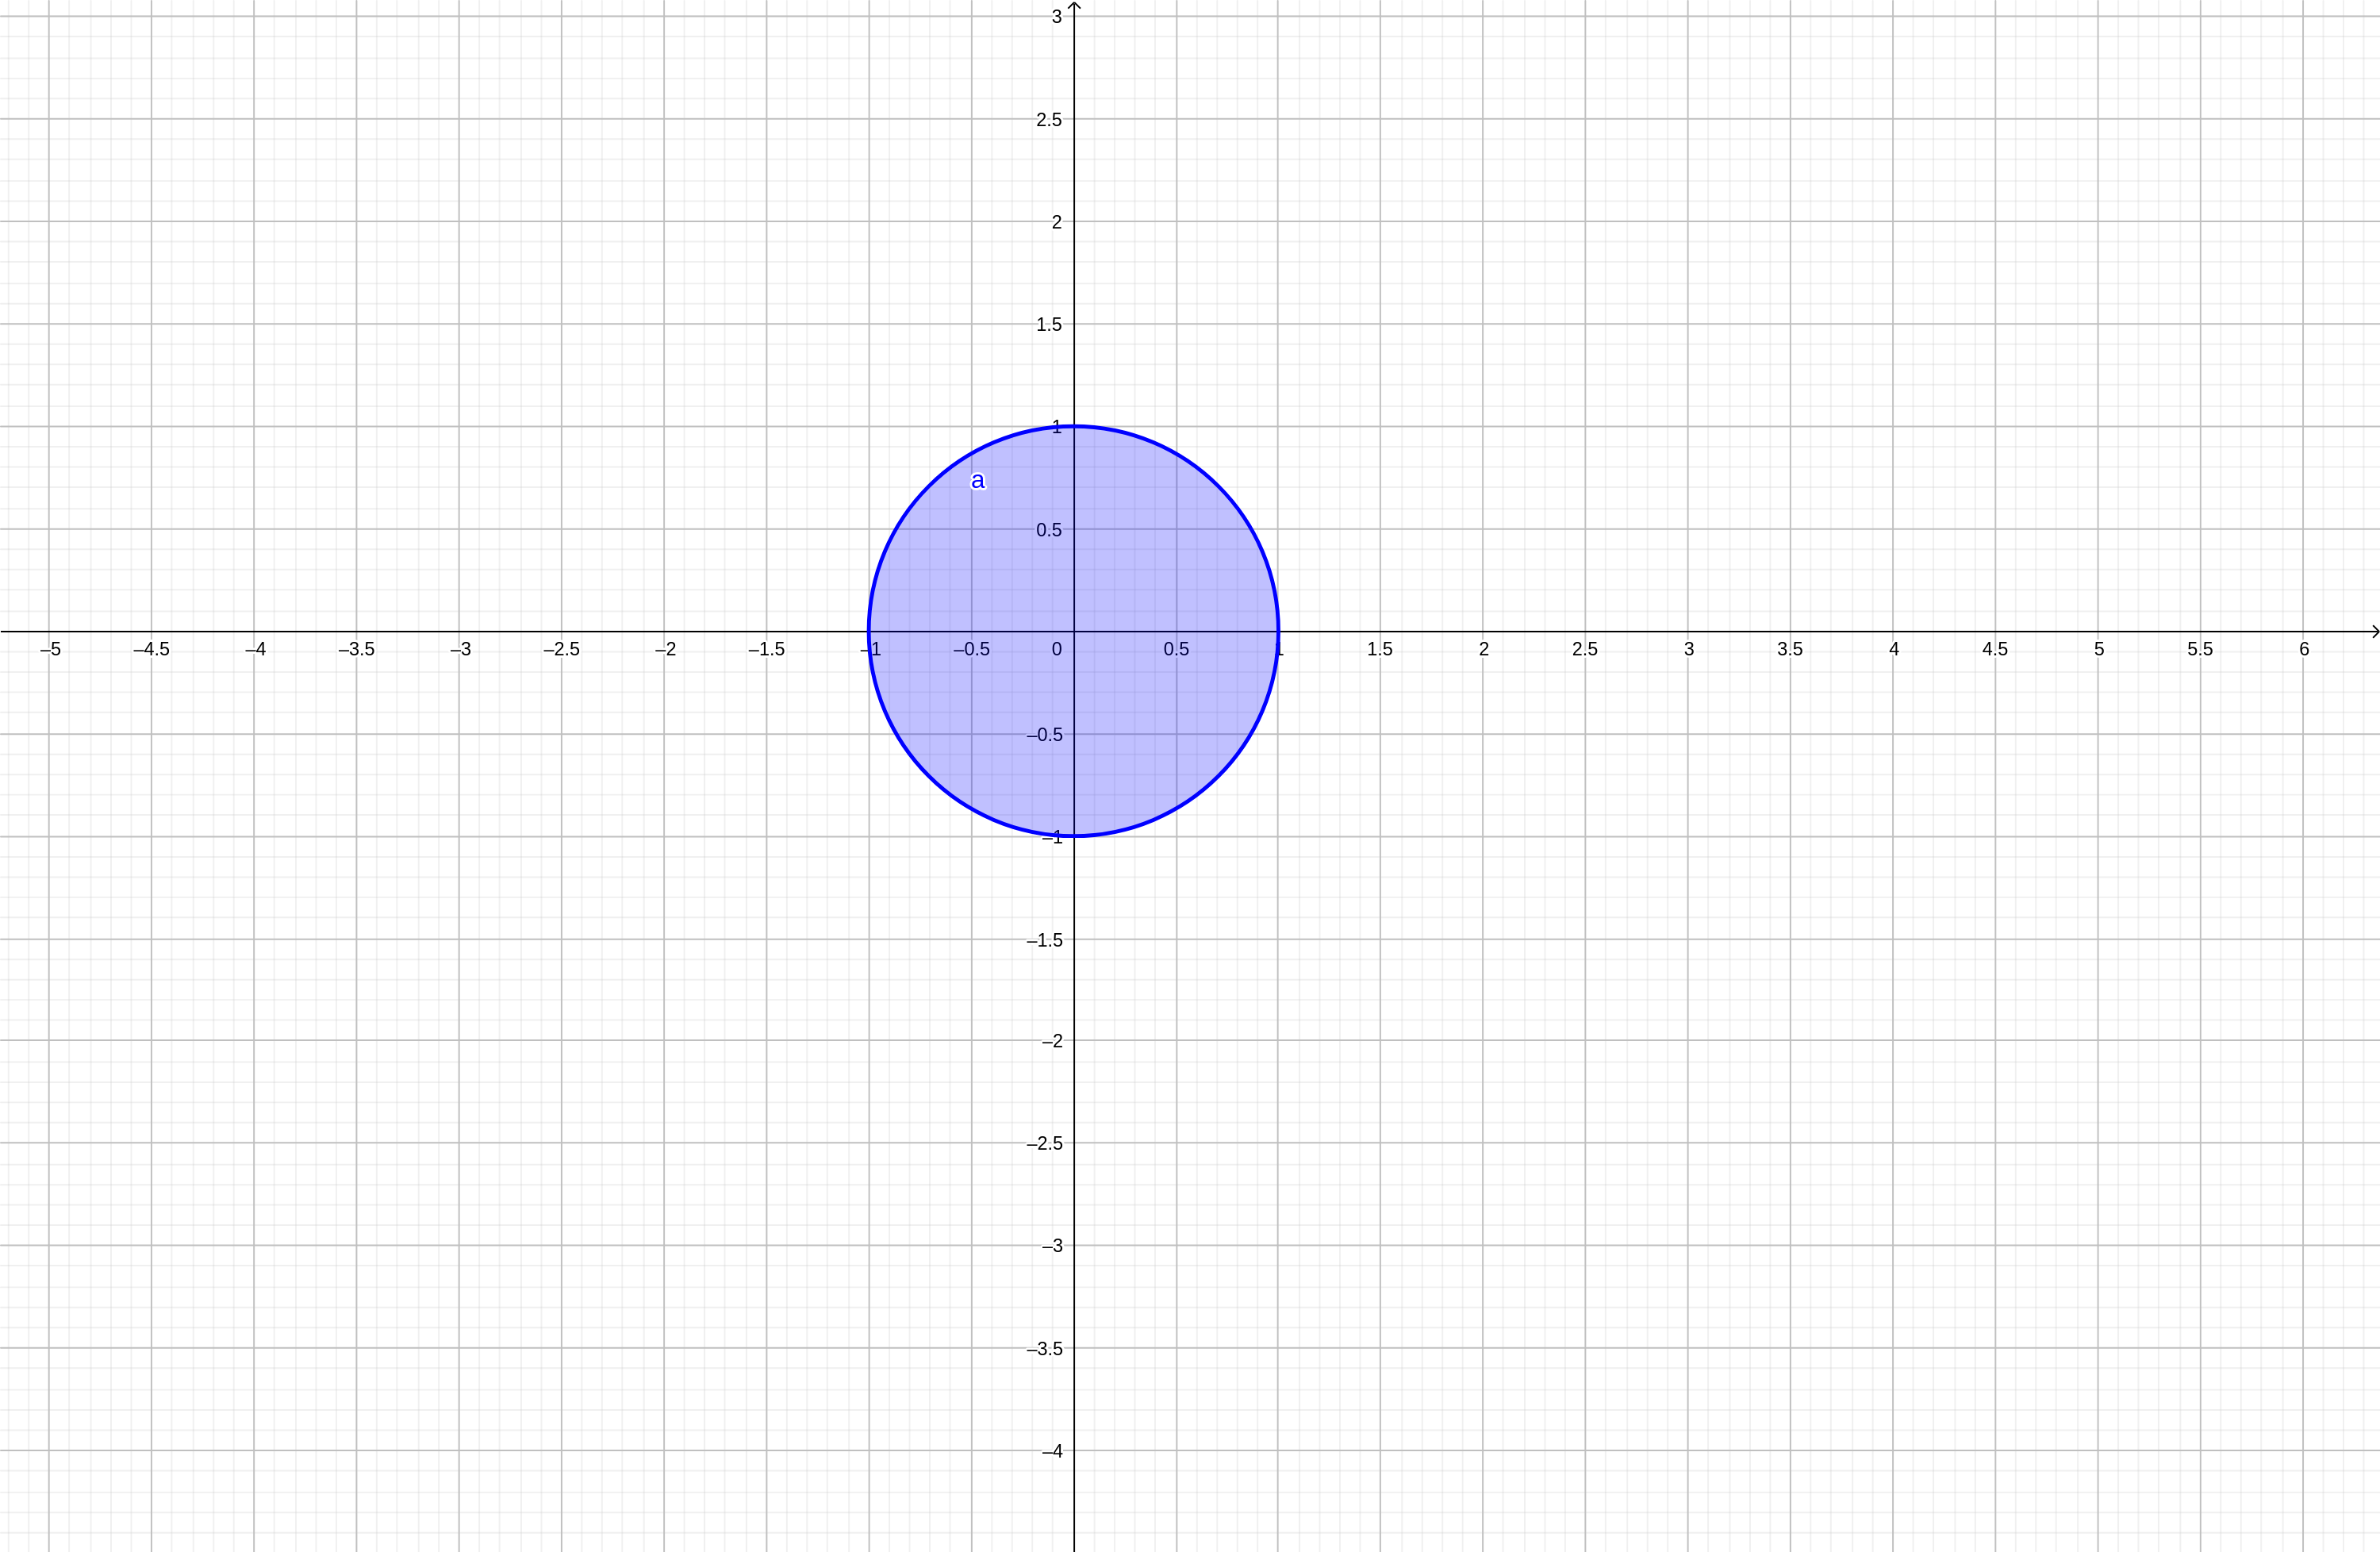
\includegraphics[width=256px]{geogebra-export.png}

\end{document}